\documentclass[12pt]{beamer}

\usepackage{ucs}
\usepackage[utf8x]{inputenc}

%\usepackage{beamerthemeBerkeley}
\usetheme{Berkeley}

\usepackage[australian]{babel}
\usepackage[T1]{fontenc}
\usepackage{graphicx}

\title{PODD Ontology Driven Database}
\author{Dr Peter Ansell}
\institute{University of Queensland}
\date{13 March 2012}

\begin{document}

\begin{frame}
\titlepage
\end{frame}


\begin{frame}
\frametitle{Background} 

\begin{itemize}
 \item PODD implemented between 2009 and 2011
 \item Design by Yuan Fang Li and Gavin Kennedy
\end{itemize}

\end{frame}

\begin{frame}
\frametitle{Motivation} 

\begin{itemize}
 \item Flexible scientific experiment management
 \item Use RDF and OWL technology to support science
\end{itemize}


\end{frame}

\begin{frame}
\frametitle{Example} 

\end{frame}

% PODD Design/Architecture as a blank slide
\bgroup
\usebackgroundtemplate{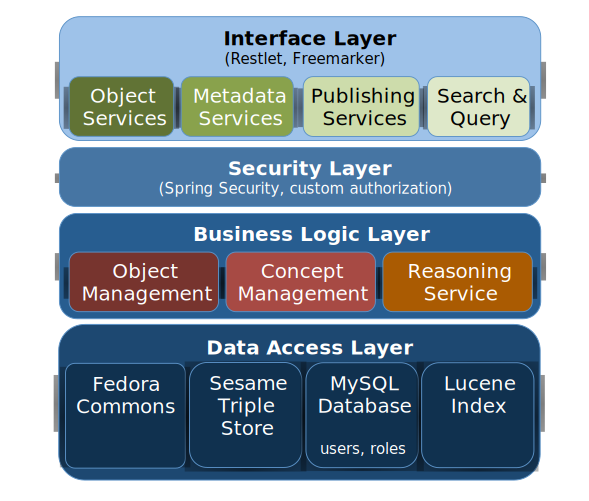
\includegraphics[
width=\paperwidth,
height=\paperheight,
keepaspectratio=true
]{podd_arch.png}}
\begin{frame}[plain]{}
\end{frame}
\egroup


% PODD Phenomics Ontology as a blank slide
\bgroup
\usebackgroundtemplate{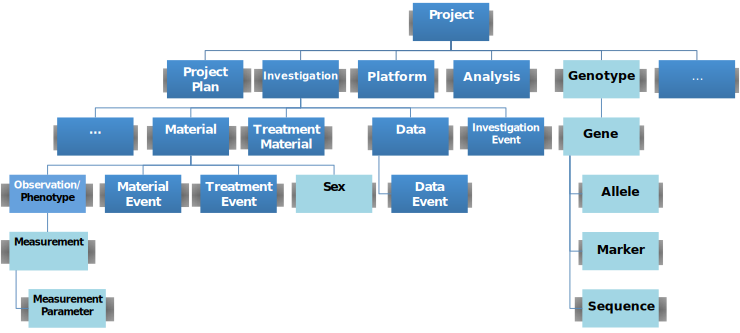
\includegraphics[
width=\paperwidth,
height=\paperheight,
keepaspectratio=true
]{podd_ont.png}}
\begin{frame}[plain]{}
\end{frame}
\egroup

\begin{frame}
\frametitle{Demo} 

\end{frame}

\begin{frame}
\frametitle{Evaluation}

Good:

\begin{enumerate}
 \item Flexible : Simultaneously support different experiments
 \item Adaptable : Additions and changes to schema ontologies
\end{enumerate}

Bad:

\begin{enumerate}
 \item Current implementation does not scale
 \item Object oriented, pulling document into memory
 \item Dependencies not supported anymore, including OWL-1.1, Fedora-3.2 and Spring-2
\end{enumerate}


\end{frame}

\begin{frame}
\frametitle{Next steps}

Redesign of the internal implementation:

\begin{itemize}
 \item Single database, currently 4 databases
 \item Only query data as needed
 \item Use upcoming SPARQL 1.1 Query and Update standards
 \item Use OWL-2
 \item Support links from experiments to other RDF documents
\end{itemize}


\end{frame}


\begin{frame}
\frametitle{Questions}

\begin{center}
Open source code can be found online at:

\url{https://github.com/podd}

\vskip 12pt

My email is: peter.ansell@uq.edu.au
\end{center}
\end{frame}

\end{document}


